\documentclass[a4paper,12pt]{extarticle}
\usepackage[utf8x]{inputenc}
\usepackage[T1,T2A]{fontenc}
\usepackage[russian]{babel}
\usepackage{hyperref}
\usepackage{indentfirst}
\usepackage{listings}
\usepackage{color}
\usepackage{xcolor}
\usepackage{here}
\usepackage{array}
\usepackage{multirow}
\usepackage{graphicx}
\usepackage{amsmath}

\hypersetup{
    colorlinks = false,
    linkbordercolor = {white}
}

\definecolor{string}{HTML}{B40000} % цвет строк в коде
\definecolor{comment}{HTML}{008000} % цвет комментариев в коде
\definecolor{keyword}{HTML}{1A00FF} % цвет ключевых слов в коде
\definecolor{morecomment}{HTML}{8000FF} % цвет include и других элементов в коде
\definecolor{сaptiontext}{HTML}{FFFFFF} % цвет текста заголовка в коде
\definecolor{сaptionbk}{HTML}{999999} % цвет фона заголовка в коде
\definecolor{bk}{HTML}{FFFFFF} % цвет фона в коде
\definecolor{frame}{HTML}{999999} % цвет рамки в коде
\definecolor{brackets}{HTML}{B40000} % цвет скобок в коде

\usepackage{caption}
\renewcommand{\lstlistingname}{Программа} % заголовок листингов кода

\bibliographystyle{ugost2008ls}

\usepackage{listings}
\lstset{ %
	extendedchars=\true,
	keepspaces=true,
	language=Python,						% choose the language of the code
	% Цвета
	keywordstyle=\color{keyword}\ttfamily\bfseries,
	%stringstyle=\color{string}\ttfamily,
	stringstyle=\ttfamily\color{red!50!brown},
	commentstyle=\color{comment}\ttfamily\itshape,
	morecomment=[l][\color{morecomment}]{\#},
	basicstyle=\footnotesize,		% the size of the fonts that are used for the code
	numbers=left,					% where to put the line-numbers
	numberstyle=\footnotesize,		% the size of the fonts that are used for the line-numbers
	stepnumber=1,					% the step between two line-numbers. If it is 1 each line will be numbered
	numbersep=5pt,					% how far the line-numbers are from the code
	backgroundcolor=\color{white},	% choose the background color. You must add \usepackage{color}
	showspaces=false				% show spaces adding particular underscores
	keywordstyle=color{blue}\bfseries, 
	showstringspaces=false,			% underline spaces within strings
	showtabs=false,					% show tabs within strings adding particular underscores
	frame=single,          		% adds a frame around the code
	tabsize=2,						% sets default tabsize to 2 spaces
	captionpos=t,					% sets the caption-position to top
	breaklines=true,				% sets automatic line breaking
	breakatwhitespace=false,		% sets if automatic breaks should only happen at whitespace
	escapeinside={\%*}{*)},			% if you want to add a comment within your code
	postbreak=\raisebox{0ex}[0ex][0ex]{\ensuremath{\color{red}\hookrightarrow\space}},
	texcl=true,
	inputpath=listings,                     % директория с листингами
}

\usepackage[left=2cm,right=2cm,
top=2cm,bottom=2cm,bindingoffset=0cm]{geometry}

%% Нумерация картинок по секциям
\usepackage{chngcntr}
\counterwithin{figure}{section}
\counterwithin{table}{section}

%%Точки нумерации заголовков
\usepackage{titlesec}
\titlelabel{\thetitle.\quad}
\usepackage[dotinlabels]{titletoc}

%% Оформления подписи рисунка
\addto\captionsrussian{\renewcommand{\figurename}{Рисунок}}
\captionsetup[figure]{labelsep = period}

%% Подпись таблицы
\DeclareCaptionFormat{hfillstart}{\hfill#1#2#3\par}
\captionsetup[table]{format=hfillstart,labelsep=newline,justification=centering,skip=-10pt,textfont=bf}

%% Путь к каталогу с рисунками
\graphicspath{{fig/}}

\begin{document}	% начало документа

% Титульная страница
%\begin{titlepage}	% начало титульной страницы

	\begin{center}		% выравнивание по центру

		Санкт-Петербургский Национально Исследовательский Университет\\
		информационных технологий, механики и оптики \\
		Кафедра систем управления и информатики\\[3cm]
		% название института, затем отступ 6см
		
		\huge \textbf{РЕФЕРАТ}\\[0.5cm]
		\large Электромеханические системы\\[0.1cm]
		\large Система автоматического управления квадракоптера Parrot ARDrone 2.0\\[2cm]

	\end{center}


	\begin{flushright} % выравнивание по правому краю
%		\begin{minipage}{0.5\textwidth} % врезка в половину ширины текста
%			\begin{flushleft} % выровнять её содержимое по левому краю

				\large Выполнили студенты группы P3335\\
				\large А.М. Зенкин\\[0.5cm]
				\large К.В. Карпов\\[0.5cm]
				
				\large Принял  к.т.н., доцент кафедры СУиР\\
				\sign[4cm]\large  М.С. Чежин\\
				\large Оценка: \sign\\
				«\underline{\hspace{0.7cm}}» \underline{\hspace{2cm}} \the\year г.

%			\end{flushleft}
%		\end{minipage}
	\end{flushright}
	
	\vfill % заполнить всё доступное ниже пространство

	\begin{center}
	\large Санкт-Петербург\\
	\large \the\year % вывести дату
	\end{center} % закончить выравнивание по центру

\thispagestyle{empty} % не нумеровать страницу
%\end{titlepage} % конец титульной страницы
\newpage


% Содержание
% Содержание
\renewcommand\contentsname{\centerline{Содержание}}
\tableofcontents
\thispagestyle{fancy}
\newpage





\section{Цель работы}
Изучить методику назначения режима резания по таблицам нормативов. Ознакомиться и приобрести навыки работы с нормативами.

\section{Варианты параметров}			
Вид заготовки и ее характеристика: Серый чугун СЧ20 $HB210;$\\

Вид обработки и параметр шероховатости: торцовое фрезерование, $Ra=1,6$, мкм\\

Модель станка: 6Р12;\\

$B=150$, мм; $l=500$, мм; $h=4$, мм;\\					
\section{Ход выполнения работы}

\subsection{Описание:}
На вертикально-фрезерном станке 6Р12 производится торцевое фрезерование плоской поверхности шириной В=150 мм, длиной l=500 мм, припуск на обработку h=4 мм. Обрабатываемый материал серый чугун СЧ20, НВ210. Заготовка предварительно обработана. Обработка окончательная, параметр шероховатости обработанной поверхности Ra=1,6 мкм.

\subsection{Выполнение эскиза обработки:}
\begin{figure}[H]
	\begin{center}
		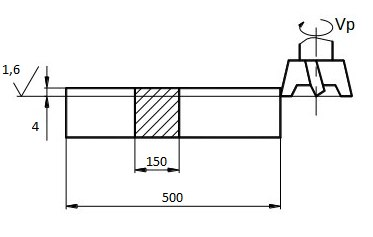
\includegraphics[scale=0.8]{1}
		\caption{Эскиз обработки} 
		\label{pic:pic_1} % название для ссылок внутри кода
	\end{center}
\end{figure}

\newpage

\subsection{Выбор инструмента:}
Для фрезерования на вертикально-фрезерном станке заготовки из чугуна выбираем торцевую фрезу с пластинками из твердого сплава ВК6, диаметром D=(1,25$\div$1,5)$\cdot$В=($1,25\div$ 1,5)$\cdot$150=$187,5\div$225 мм. Принимаем D=200 мм; z=20, ГОСТ 9473-80.\\
   Геометрические параметры фрезы: $\phi$ =$60^{\circ}$, $\alpha=12^{\circ}$, $\gamma=10^{\circ}$, $\lambda=20^{\circ}$, $\phi_1=5^{\circ}$.\\
Схема установки фрезы – смещенная.

\subsection{Режим резания:}
\subsubsection{Глубина резания:}
Заданный припуск на чистовую обработку срезают за один проход, тогда:\\
\begin{equation}
	\begin{split}
		&t=h=4\;mm;
	\end{split}
\end{equation}

\subsubsection{Назначение подачи:}
Для получения шероховатости Ra=1,6 мкм подача на оборот $S_0$=1,1$\div$2,1 мм/об\\
\begin{equation}
	\begin{split}
		&S_z=\dfrac{S_0}{z} = \frac{2}{20}\ = 0,1\;mm/dent;
	\end{split}
\end{equation}

\subsubsection{Период стойкости:}
Для фрез торцевых диаметром от 200 мм до 250 с пластинками из твердого сплава применяют период стойкости:\\
\begin{equation}
	\begin{split}
		&T=240\;min;
	\end{split}
\end{equation}

\subsubsection{Скорость резания, допускаемая режущими свойствами инструмента:}
Для обработки серого чугуна фрезой диаметром от 200 до 250 мм, глубина резания t до 4 мм, подаче до 0,1 мм/зуб.:
\begin{equation}
	\begin{split}
		&V=148,38\;m/min;
	\end{split}
\end{equation}

С учетом поправочных коэффициентов:
\begin{equation}
	\begin{split}
		&K_{MV}=0,88,\; K_{NV}=1,\; K_{IV}=1;\\
		&V=V\cdot K_{MV}\cdot K_{NV}\cdot K_{IV}=1\cdot 1\cdot 148,38 = 130,57\; m/min;\\
	\end{split}
\end{equation}

Частота вращения шпинделя, соответствующая найденной скорости резания:
\begin{equation}
	\begin{split}
		&n=\dfrac{1000\cdot V}{\pi \cdot D}=\dfrac{1000\cdot 130,57}{3,14\cdot 200}=207,81\; rpm;\\
	\end{split}
\end{equation}

Корректируем по паспорту станка:
\begin{equation}
	\begin{split}
		&n=200\; rpm;\\
	\end{split}
\end{equation}

Действительная скорость резания
\begin{equation}
	\begin{split}
		&V_p=\frac{\pi \cdot D\cdot n}{1000}=\frac{3,14 \cdot 200\cdot 200}{1000}=125,6\; m/min;\\
	\end{split}
\end{equation}

\subsubsection{Минута подачи:}
\begin{equation}
	\begin{split}
		&S_M=S_z\cdot z\cdot n =0,1\cdot 20\cdot 200 = 400\;mm/min;\\
	\end{split}
\end{equation}
Это совпадает с паспортными данными станка.

\subsection{Мощность:}
\subsubsection{Мощность, затрачиваемая на резание:}
При фрезеровании чугуна с твердостью до НВ210, ширине фрезерования до 150 мм, глубине резания до 4 мм, подаче на зуб 0,1 мм/зуб, минутной подаче 400 мм/мин
\begin{equation}
	\begin{split}
		&N_p=11,75\;kW;\\
	\end{split}
\end{equation}

\subsubsection{Проверка достаточности мощности станка:}
Мощность на шпинделе станка: $N_{spindel}=N_d\cdot \eta;$

\begin{equation}
	\begin{split}
		&N_d=7,5\;k/W;\; \eta=0,8;\\
		&N_{sp} = 7,5\cdot 0,8 = 6\;kW;\\
	\end{split}
\end{equation}

Так как $N_{sp}=6 \;kW\; <\; N_p=11,75\;kW$, то обработка невозможна.\\

\subsection{Основное время:}
\begin{equation}
	\begin{split}
		&T_0=\frac{L}{S_M};\\
	\end{split}
\end{equation}
где $L=l+l_1;$\\

Расчёт основного времени не производится, так как мощность на шпинделе станка меньше требуемой мощности.\\

\section{Вывод}
В данной лабораторной работе была изучена методика назначения режима резания по таблицам нормативов. Также были получены навыки работы с номативами. Был построен эскиз обработки (рис. \ref{pic:pic_1}).
\end{document}